\chapter{Introduction}
\label{cha:introduction}

The main objective of presented project is the implementation of parts of 3D engine in a browser environment. Parts of engine are analysed side-by-side with parallel engine compiled from C++. The objective of analysis is comparison of performance and description of possible issues related to the limited browser resources and dynamic features of JavaScript.

At the moment of writing majority of games are developed with C++ and usually DirectX. These technologies are mature and have excellent performance. Features of the language give flexibility and high-level solutions to effectively manage application (e.g. operator overloading, multiple inheritance) and allow to fine-tune internals of application to achieve best execution times. For games with high budget\footnote{Grand Theft Auto V, released in 2013 had a budget of \$137 millions -- http://www.gamesindustry.biz/articles/2013-02-01-gta-v-dev-costs-over-USD137-million-says-analyst} C++ is an obvious choice for having the best possible result.

However, in parallel to AAA game industry casual and independent games sector is growing. In 2013 market is expected to be worth \$8.64 billions in total. Total of 2.4 billion tablets and smartphones with casual games capabilities will be reached before the end of 2013. These games are less focused on creating cutting edge graphics and physics simulations and more on overall experience and social interactions.

JavaScript is a scripting language not designed to perform high-load computations. However, at present it is the only language widely supported by all browsers. With all it's advantages and quirks is the only choice available for programmers.\footnote{Currently two new languages are worked on -- Dart by Google and TypeScript by MicroSoft. However, to enable cross-compilation to JavaScript, paradigm of these languages is similar and work is focused mainly on better IDE support.}

While suffering from design issues, JavaScript provides a complete environment that makes development very easy for both beginner and advanced programmer. Two very important components of every application are provided out of the box -- rendering system and networking in browser, designed for HTML pages to carry mainly text information are still suitable for gaming. Creation of simple 2D game is often a matter of few hundred lines of code responsible for transferring user input to positions of sprites defined in CSS. This is clearly visible during competitions like JS13kGames\footnote{http://js13kgames.com/} where all game assets and code have to be fitted into 13kB package.

Many projects varying from server side solutions\footnote{http://nodejs.org/}\footnote{http://googlecreativelab.github.io/coder/} to hardware developer boards\footnote{http://www.espruino.com/} are taking advantage of this simplicity. From the perspective of game development, it is unlikely at the time of writing that AAA game may be created to run in browser. However, growing segments of casual, independent and social games are already targeting web as a platform.

\section{Influence on distribution process}

Traditionally, games are often still sold in physical boxes and some update system is always incorporated to patch any bugs appearing after initial release. Systems like Steam\footnote{http://store.steampowered.com/} are making this process easier but still suffer from necessity to install a game on hard drive.

Creating application that works in browser simplifies distribution significantly. All assets and code are downloaded each time user enters a website, so no update system is necessary -- all users always play the newest version. Usually browser games are monetised differently than traditional titles. Playing basic version is usually free and earnings come from either ads or premium content. This is completely new approach, present also in MMO\footnote{Massive Multiplayer Online} games. It resulted in psychological research on leveraging compulsive behaviours to maximise profits\footnote{http://www.emcneill.com/exploitative-game-design-beyond-the-f2p-debate/}.

Working in browser gives access to all social network of user, so incorporation of Twitter or Facebook based features is very simple -- which boosts promotion of game. It also enables, morally questionable, target of people not able to install games on company issued computer. Disallowing games in browsers is far more complicated task for administrator, similar to blocking ads or mature content.

Lastly, web is better suited to run easily on all platforms. Browser is a layer of abstraction that makes transparent for application, whether it runs on any traditional operating system, gaming console or mobile device. Of course  performance and screen size should be taken under consideration, but ability to write one codebase that runs on multiple devices led already to projects that package JavaScript applications as native ones\footnote{http://phonegap.com/}, greatly reducing development costs for growing variety of phones and tablets.

\begin{figure}[h!]
  \caption{Game created with ImpactJS}
  \label{img:impactjs}
  \centering
	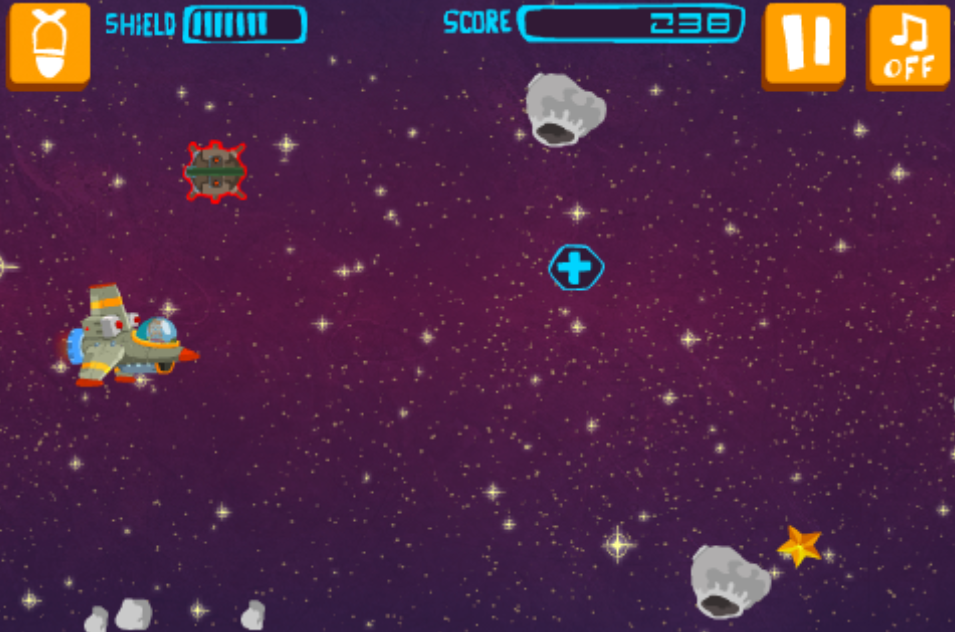
\includegraphics[width=12cm]{summary/impactjs.png}
\end{figure}

Multiple open-source and commercial game engines are created lately. Examples worth mentioning are ImpactJS\footnote{http://impactjs.com/}, Turbulenz\footnote{http://biz.turbulenz.com/turbulenz} and Isogenic Engine\footnote{http://www.isogenicengine.com/}.


\begin{figure}[h!]
  \caption{Game created with Isogenic Engine}
  \label{img:isogenic}
  \centering
	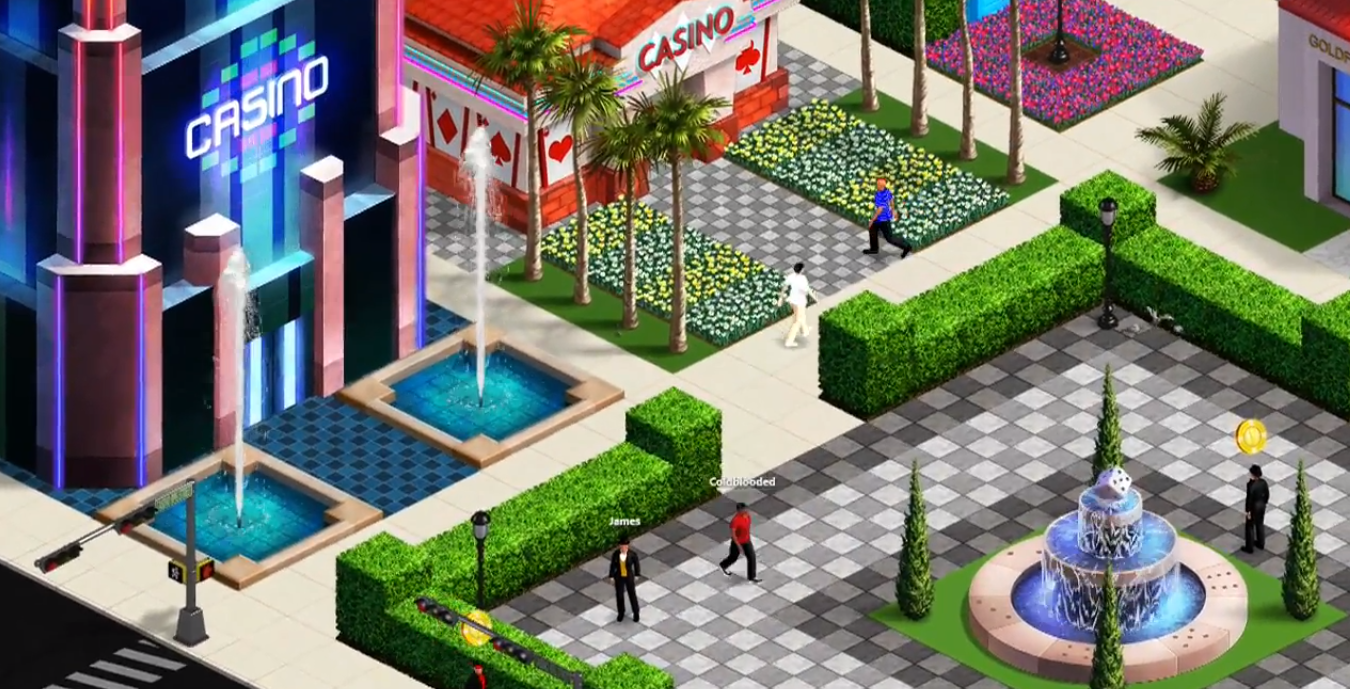
\includegraphics[width=12cm]{summary/isogenic.png}
\end{figure}

Very important and growing sector are interactive 3D arts with two major targets -- music videos and commercials. They are uniquely available only in browsers as a very viral extensions of normal marketing. One of the first occurrences of this technology was video for Rome music group: "3 dreams of black"\footnote{http://www.ro.me/}. Project allows to move the camera while animated 3D story is rendered alongside music. After movie is over user is allowed to create 3D models that are later incorporated into experiences of other people watching. This way interactions and social element are enabled in what used to be one-way transmission of art form.

\begin{figure}[h!]
  \caption{Screenshot from "3 dreams of black"}
  \label{img:rome}
  \centering
	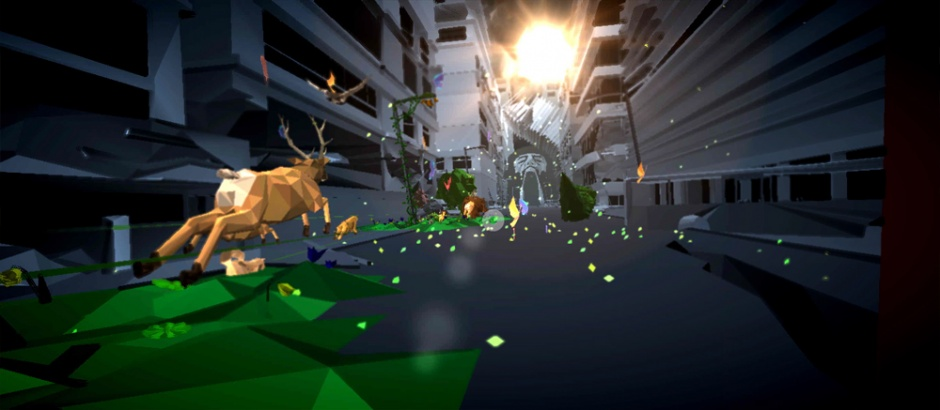
\includegraphics[width=12cm]{summary/rome.jpg}
\end{figure}

\section{Technology}

Browser-based engine is implemented in JavaScript and analyzed in V8 engine. V8 is maintained by Google and is used in Google Chrome browser. Executable examples are compiled using gcc compiler and are runned on the same platform. For additional comparison Emscripten project is used to automatically generate JavaScript and measure if automated conversion may be as effective as writing code by hand.

Project is based on conference sessions and announcements authored by V8 programmers regarding performance of JavaScript applications. Analysis of available materials is a topic of Chapter 2, where internals of modern engines for dynamic languages are briefly explained.

Chapter 3 covers particles often used to simulate loosely connected systems like smoke, fire, fog, etc. It shows techniques of memory allocation and garbage collection that help improve performance. Two particle systems are presented -- one with high memory allocation that is expected to cause performance issues and second one, improved by usage of object pools.

Chapter 4 is focused on sphere collision detection and reaction, with both naive solution and space partitioning using Octree. This benchmark shows application with high CPU usage and relatively simple math computations. Because of this simplicity, collision detection with spheres is almost always used as a preliminary method of eliminating collision between objects. Only if bounding spheres are colliding more complex and expensive algorithms are used to determine real state of such pair.

Systems presented in chapters 3 and 4 are not targeted to be full physics engines. They are however representative to general concepts encountered in every game.

Chapter 5 describes Emscripten, project aimed to convert complete C++ projects to JavaScript. Related library, asm.js, is presented with overview of architectural choices that lead to better performance. Generated code is compared to the one created in previous chapters and execution times of all benchmarks is compared and briefly explained.

Last chapter is summary of all achieved results. Limitations of JavaScript engines are presented alongside future possibilities for gaming industry. 

Benchmarks are by no means a complete physics system and are not representing current state of the art of physics algorithms. They are aimed to resemble optimal algorithms in used methods and complexity, so that benchmarks reflect how actual engine is using memory and computing power.

